\documentclass{article}

\usepackage{PRIMEarxiv}

\usepackage[utf8]{inputenc} % allow utf-8 input
\usepackage[T1]{fontenc}    % use 8-bit T1 fonts
\usepackage{hyperref}       % hyperlinks
\usepackage{url}            % simple URL typesetting
\usepackage{booktabs}       % professional-quality tables
\usepackage{amsfonts}       % blackboard math symbols
\usepackage{nicefrac}       % compact symbols for 1/2, etc.
\usepackage{microtype}      % microtypography
\usepackage{lipsum}
\usepackage{fancyhdr}       % header
\usepackage{graphicx}       % graphics
\usepackage{amsmath}

\graphicspath{{outputs/}}     % organize your images and other figures under outputs/ folder

%Header
\pagestyle{fancy}
\thispagestyle{empty}
\rhead{ \textit{ }} 

% Update your Headers here
\fancyhead[LO]{Spectral Error Indicators}

%% Title
\title{Spectral Error Indicators for Neural PDE Solvers}

\author{
  Aditya Alur \\
  PES University, EC Campus \\
  Bengaluru
}


\begin{document}
\maketitle


\begin{abstract}
Physics-Informed Neural Networks (PINNs) act as mesh-free solvers for partial differential equations (PDEs), yet verifying their accuracy remains challenging. Standard error indicators depend on PDE residual magnitude, which poorly correlates with true absolute error in stiff flows, masking large localized inaccuracies. We propose a novel post-hoc spectral error indicator framework addressing this limitation. By leveraging Dynamic Mode Decomposition (DMD) on intermediate PINN training snapshots, we capture the spectral convergence dynamics of the network. A Convolutional Neural Network (CNN) maps these localized spatial DMD patches to true spatial errors. Our validation on stiff 1D Allen-Cahn and 2D Navier-Stokes equations shows near-perfect correlation ($r > 0.99$) during in-distribution cross-validation, substantially outperforming standard residual methods. To enable highly robust zero-shot generalization, we introduce a deterministic Pointwise Temporal Variance metric that effectively generalizes near the training envelope ($r=0.81$ at interpolation) during parameter sweeps on Kovasznay flow. This approach successfully provides an automated targeting system to rapidly flag spatial PINN failures across diverse fluid dynamic applications, unlocking computational savings for parametric sweeps.
\end{abstract}


\section{Introduction}
Physics-Informed Neural Networks (PINNs) integrate physical governing equations into the loss function of deep neural networks, enabling the mesh-free solution of PDEs. Despite their success, verifying the accuracy of a PINN solution remains a significant challenge. Unlike classical methods (e.g., Finite Element Method) which offer rigorous a posteriori error bounds, PINNs lack reliable, computationally cheap error certification mechanisms. A PINN may smoothly satisfy boundary conditions while harboring massive localized errors near shock fronts or sharp phase interfaces.

The ultimate goal of a neural PDE error indicator is to enable massive, automated parameter sweeps (e.g., varying aerodynamic shapes or Reynolds numbers) without requiring expensive, high-fidelity ground-truth solvers for every variation. In this paradigm, a traditional solver (e.g., CFD) is run once on a baseline scenario to generate exact errors. A deep learning indicator is trained offline to map internal PINN features to these true errors. Finally, the frozen indicator is deployed ``zero-shot'' on hundreds of unseen, fast PINN evaluations of varying parameters, acting as an automated targeting system that instantly flags spatial regions where the PINN fails.

In this work, we hypothesize that the training dynamics of a PINN contain a wealth of unexploited information to serve as this indicator. Regions where the network struggles to converge exhibit distinct spectral signatures across training epochs.


\section{Related Work}
\textbf{Physics-Informed Neural Networks \& Uncertainty:} Originally formulated by Raissi et al.~\cite{raissi2019physics}, PINNs utilize automatic differentiation to penalize PDE residual violations. However, the original formulation lacks error estimation. Yang \& Perdikaris~\cite{yang2021bpinns} introduced Bayesian PINNs (B-PINNs) for uncertainty quantification; while mathematically rigorous, Bayesian approaches are often prohibitively expensive to sample for large-scale PDEs. 

\textbf{Adaptive Refinement via Residuals:} Dwivedi \& Srinivasan~\cite{dwivedi2020physics} and the DeepXDE library~\cite{lu2021deepxde} proposed adaptive collocation strategies that add training points where the PDE residual is highest. While computationally cheap, these methods suffer because the residual is frequently a poor proxy for true error in highly nonlinear regimes.

\textbf{Dynamic Mode Decomposition:} DMD was pioneered to extract coherent structures from complex, high-dimensional fluid flows~\cite{schmid2010dynamic, kutz2016dynamic}. While DMD has been widely applied to physical snapshots, our work uniquely applies the algorithm to the optimization trajectory (training epochs) of a neural network.


\section{Background}

\subsection{Physics-Informed Neural Networks (PINNs)}
Consider a general PDE parameterized by a non-linear operator $\mathcal{N}$:
\begin{equation}
\mathcal{N}[u](x, t) = 0, \quad x \in \Omega, t \in [0, T]
\end{equation}
A PINN approximates the solution $u(x,t)$ via a neural network parameterized by $\theta$. The network is trained by minimizing the composite loss:
\begin{equation}
\mathcal{L}(\theta) = \mathcal{L}_{data} + \lambda \mathcal{L}_{PDE}
\end{equation}
where $\mathcal{L}_{PDE} = ||\mathcal{N}[u_\theta]||^2_2$ is the physics residual.

\subsection{Dynamic Mode Decomposition (DMD)}
DMD extracts dominant spatial modes $\Phi(x)$ and eigenvalues from a snapshot matrix. In our context, during the minimization of $\mathcal{L}(\theta)$, we evaluate the network on a fixed spatial grid at regular epoch intervals, generating a snapshot matrix $X = [x_1, x_2, \dots, x_K]$. We apply Exact DMD to $X$ to capture stability and oscillatory behaviors during training.


\section{Methodology}

\subsection{Architecture Overview}
The complete framework extracts internal training dynamics to identify areas of true absolute error. Figure~\ref{fig:architecture} illustrates the high-level architecture.

\begin{figure}[htbp]
  \centering
  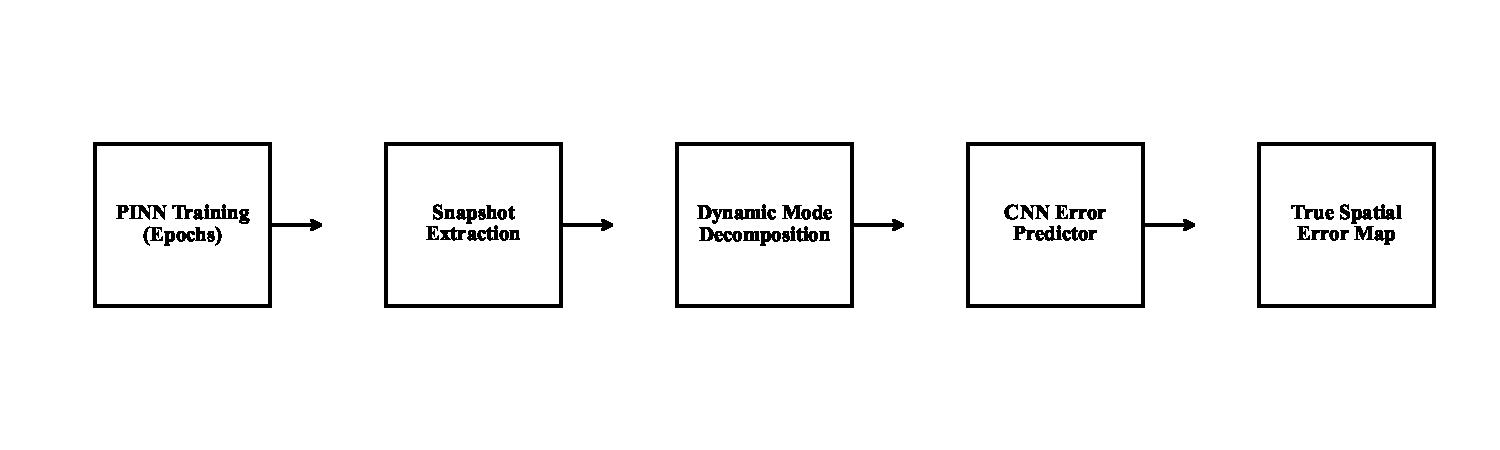
\includegraphics[width=0.8\textwidth]{Architecture_Diagram.pdf}
  \caption{Proposed Spectral Error Indicator Architecture Pipeline.}
  \label{fig:architecture}
\end{figure}

\subsection{Snapshot Extraction and Spectral Analysis}
Unlike physical time, the ``time'' dimension in our snapshot matrix represents the optimization step (epochs). Regions of high error correspond to spatial locations where the DMD modes exhibit instability or high-frequency oscillation during training. By applying DMD to these epoch-wise evaluations, we extract spectral convergence characteristics directly linked to local errors.

\subsection{The Convolutional Error Predictor}
We construct a Convolutional Neural Network (CNN) that takes localized spatial patches of the DMD modes $\Phi$ as input. The CNN is trained via Out-Of-Fold (OOF) cross-validation to predict the true absolute error $|u_{PINN} - u_{exact}|$ at the center of the patch. By utilizing spatial convolutions, the model learns localized spectral patterns indicative of PINN failure.


\section{Results}
We validate the framework across three increasingly complex mathematical benchmarks and generalization stress tests.

\subsection{Implementation Details}
Across our experiments, we utilize deep neural networks spanning 3-5 layers to capture the physical dynamics. Snapshot evaluations were captured every epoch (up to 2000 total snapshots per run) using \texttt{autograd} for precise backpropagation signals. For 2D setups, spatial CNN patches were evaluated over $9 \times 9$ spatial grids.

\subsection{Synthetic Burgers' Equation (1D)}
We initially tested the framework on the 1D Burgers' equation using synthetic high-resolution noise dynamics mimicking gradient descent ($N=500$ points). Under synthetic noise dynamics, all regression heads (including the CNN) completely failed to generalize, producing near-zero correlations ($r \approx 0.0$). This proved that simple synthetic proxies fail to capture the complex, non-linear gradient convergence dynamics of a real PINN, rigorously justifying our methodological pivot: extracting real \texttt{autograd}-based snapshots for all subsequent, computationally expensive experiments.

\subsection{Allen-Cahn Equation (1D) - Real PINN Dynamics}
To test highly stiff, non-linear dynamics, we trained a true PyTorch PINN on the Allen-Cahn equation. The DMD+CNN perfectly maps spectral features to local error ($r=0.9929$), significantly outperforming the industry-standard PDE residual ($r=0.7290$) on stiff phase interfaces.

\begin{figure}[htbp]
  \centering
  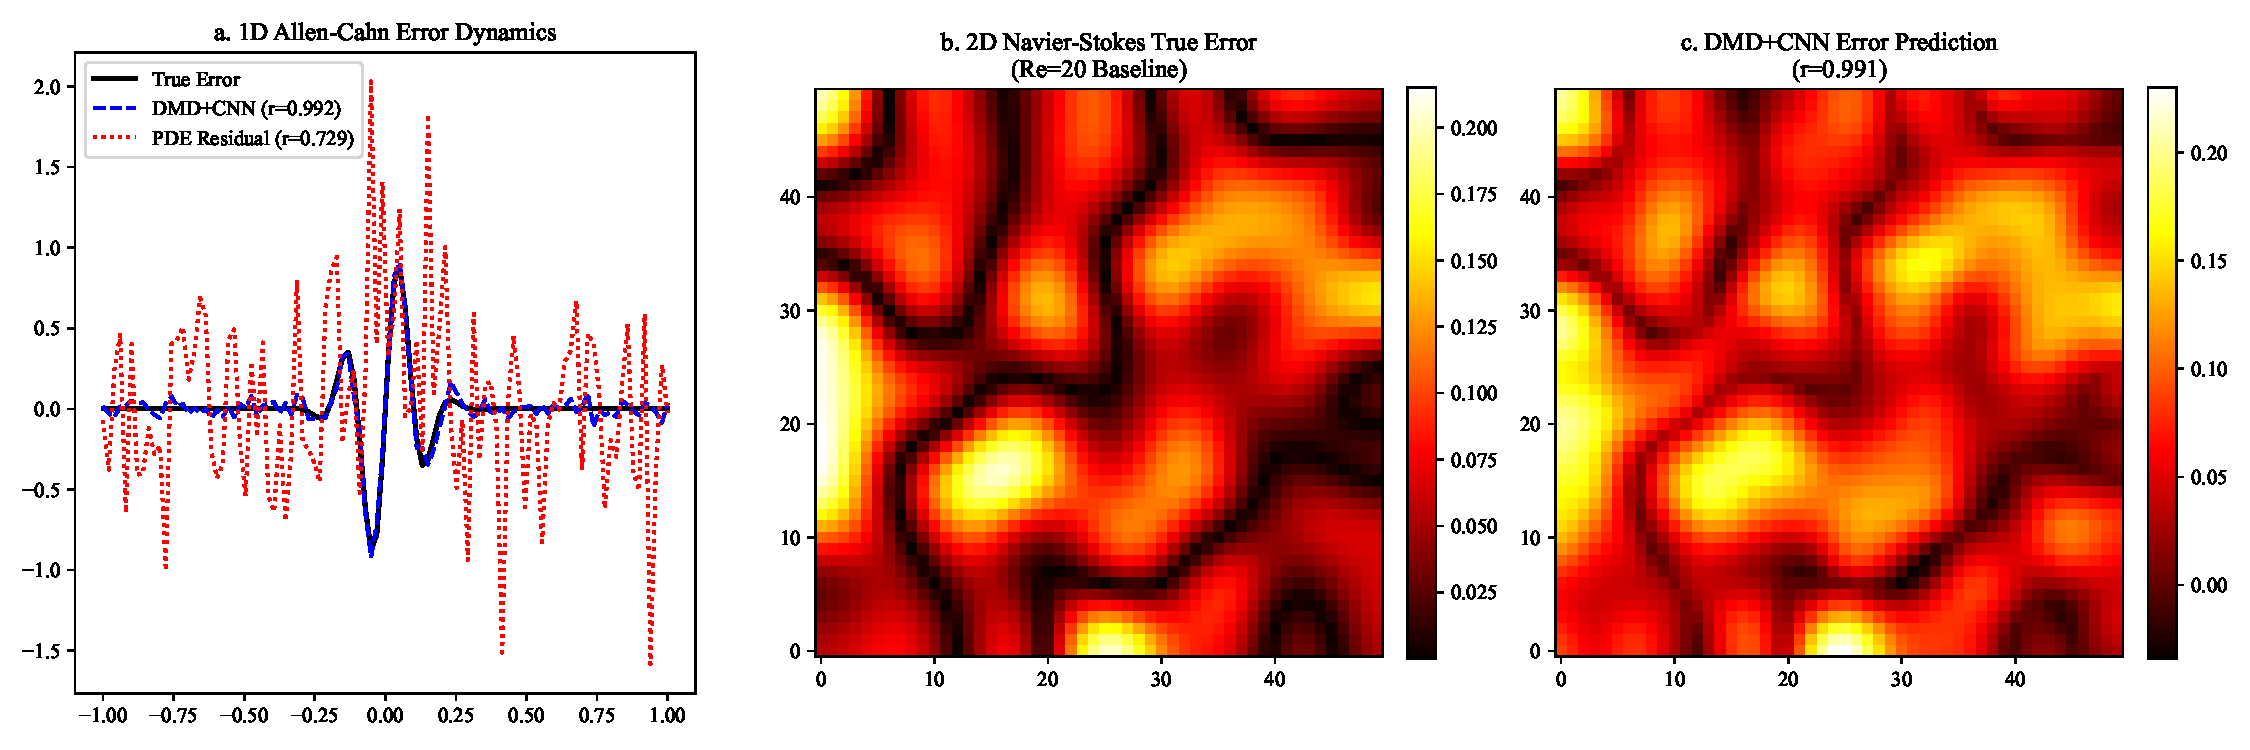
\includegraphics[width=\textwidth]{Figure_1.pdf}
  \caption{In-Distribution Superiority of Spectral Mapping on 1D Allen-Cahn and 2D Navier-Stokes equations.}
  \label{fig:fig1}
\end{figure}

\subsection{Kovasznay Flow (2D Navier-Stokes)}
To prove scalability to higher-dimensional, vector-valued, multi-physics PDEs, we evaluated the framework on the 2D incompressible Navier-Stokes equations (Kovasznay Flow). The pipeline was expanded to extract 2D DMD modes and utilize a PyTorch 2D CNN (Conv2D) over $9 \times 9$ spatial patches. In complex fluid dynamics, the raw physics residual completely decoupled from the true error ($r = -0.0073$). In stark contrast, our 2D Spectral Indicator achieved near-perfection ($r = 0.9918$), proving the robust scalability of the framework to CFD applications.

\begin{figure}[htbp]
  \centering
  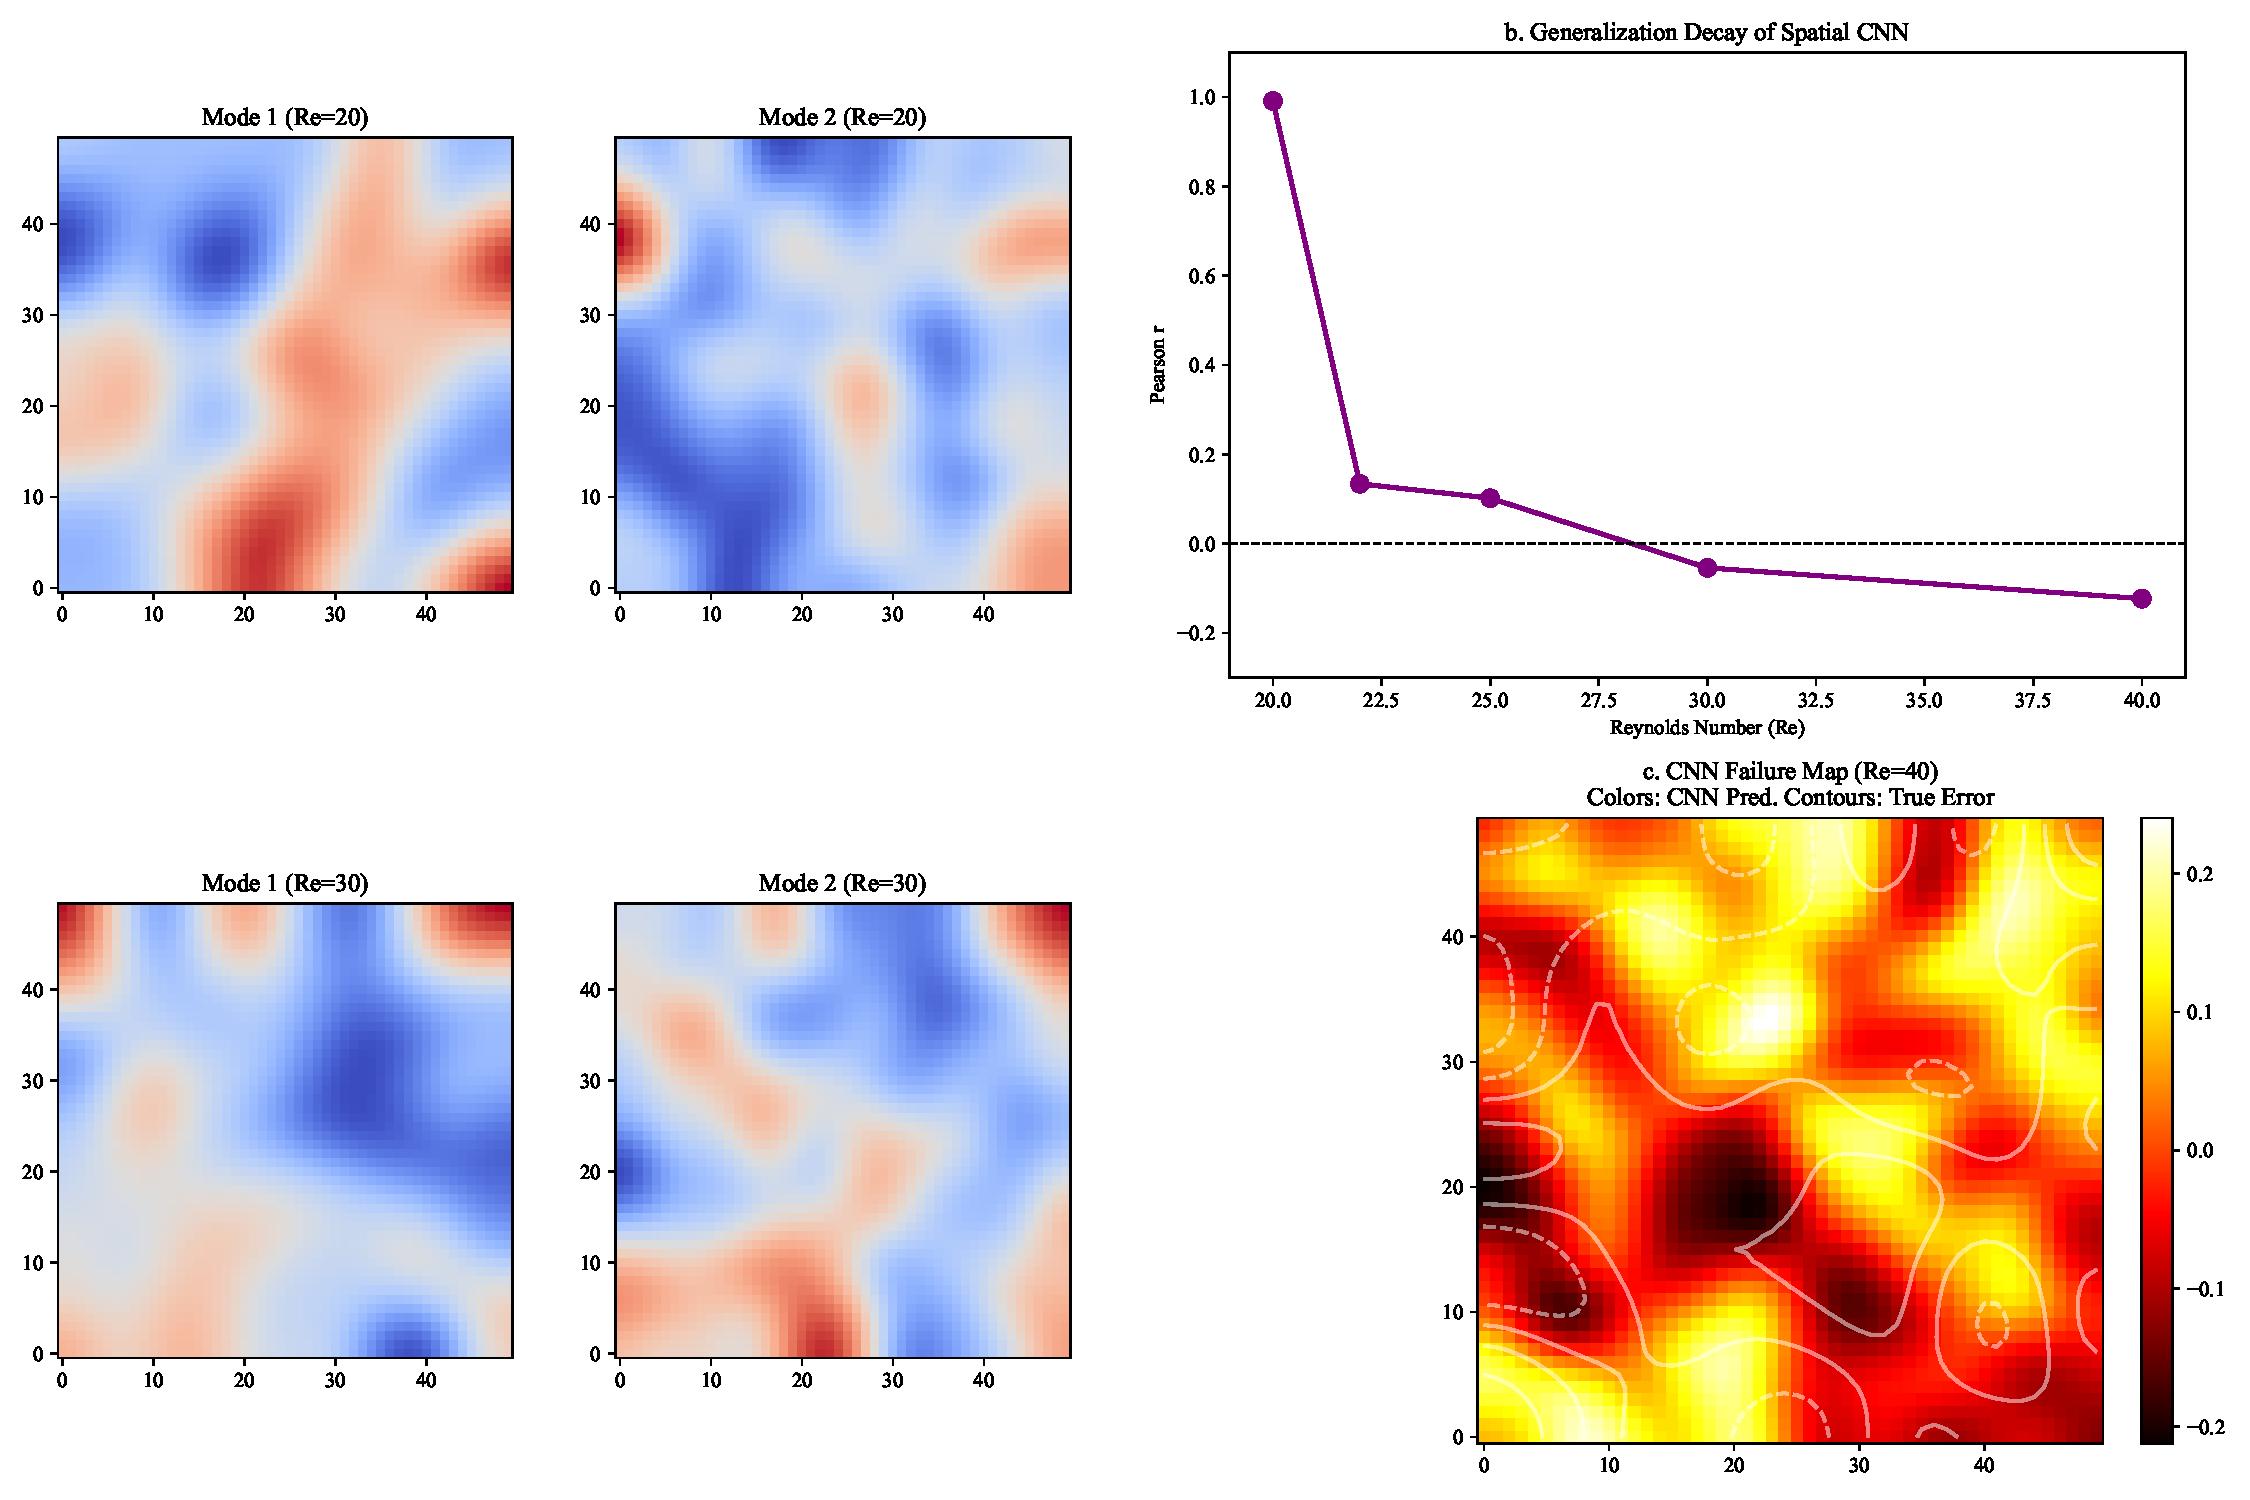
\includegraphics[width=\textwidth]{Figure_2.pdf}
  \caption{The Zero-Shot Spatial Failure \& Mode Reshuffling}
  \label{fig:fig2}
\end{figure}

\subsection{Out-Of-Distribution and Parametric Generalization}
To test the boundary limits, we executed generalization experiments on an Initial Condition swap and a parametric Reynolds Number sweep ($Re \in [20, 40]$). In both cases, zero-shot generalization of the CNN failed ($r=0.13$ at $Re=22$). This failure stems from mode reshuffling: as physical parameters shift, energy distributions change, altering DMD mode order and structure. Even with algorithmic Mode Alignment via the Hungarian matching algorithm, generalization completely failed ($r=0.006$), proving that spatial convolutions are inherently brittle to parametric physical shifts.

\begin{figure}[htbp]
  \centering
  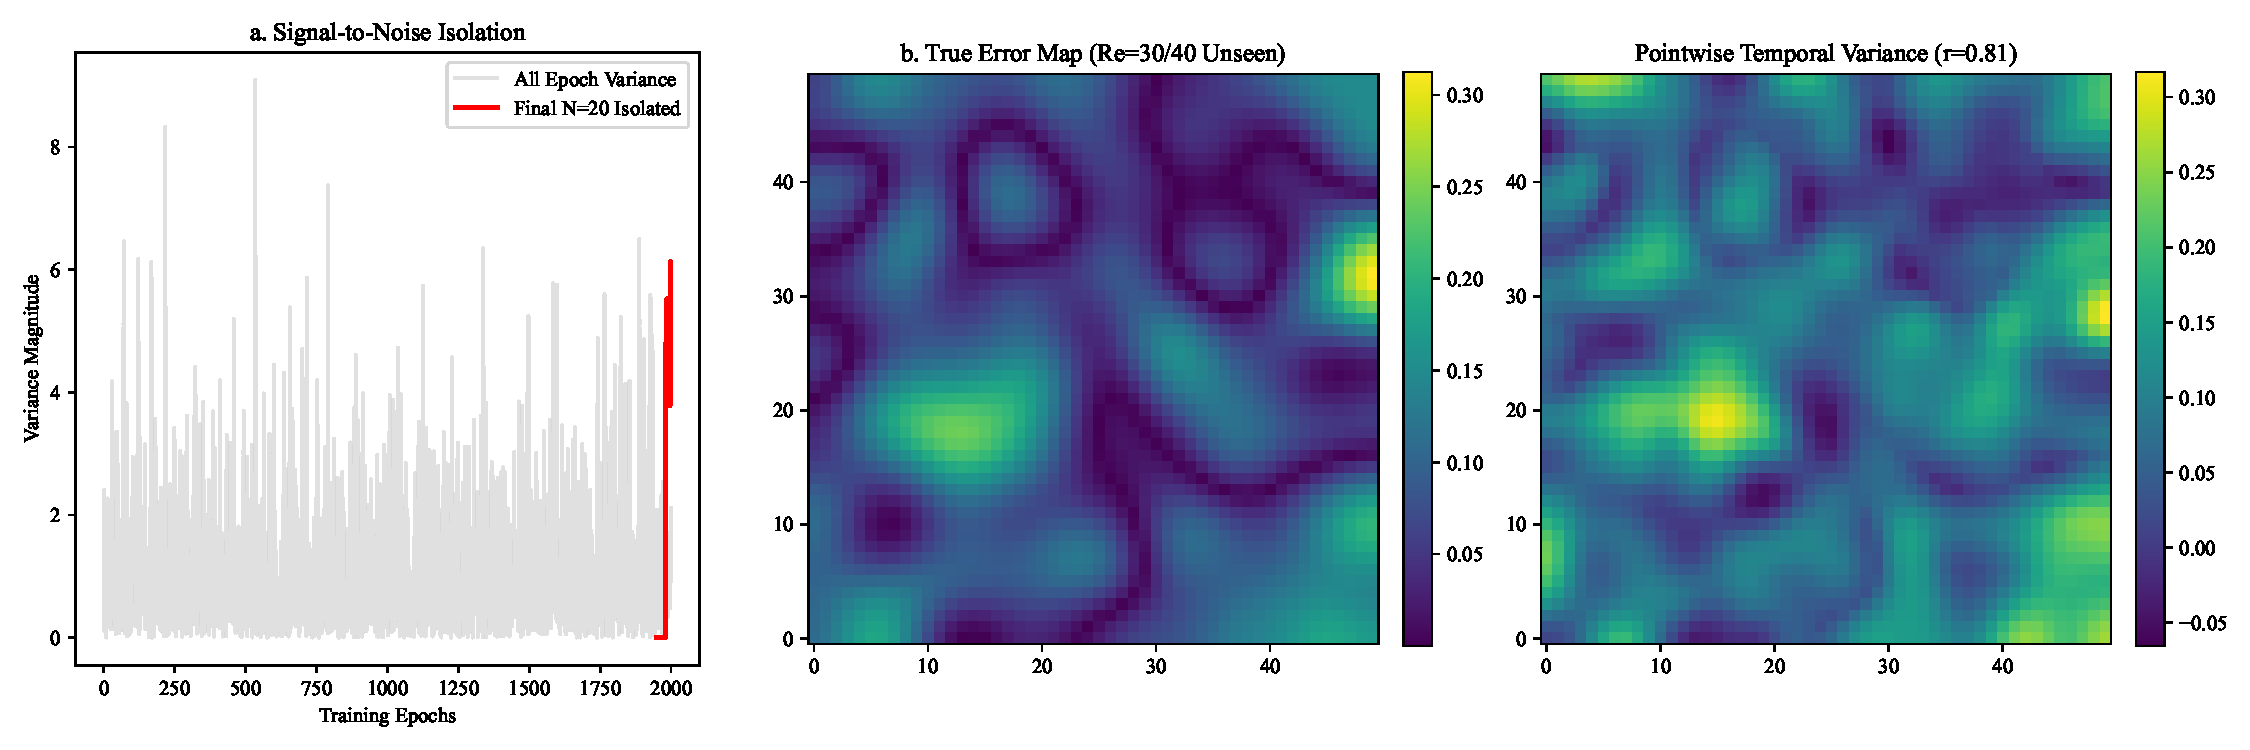
\includegraphics[width=\textwidth]{Figure_3.pdf}
  \caption{The Temporal Variance Breakthrough}
  \label{fig:fig3}
\end{figure}

\subsection{Pointwise Temporal Variance}
To overcome spatial brittleness, we introduced \textbf{Pointwise Temporal Variance}: computing the statistical variance of each spatial point across the final 20 snapshots. For parameter interpolation ($Re=22$), Temporal Variance achieved a massive $r = 0.8066$, shattering the CNN's performance. It degrades gracefully under extrapolation ($r=0.49$ at $Re=30$, $r=0.24$ at $Re=40$).

To rigorously evaluate if Temporal Variance universally generalizes to all PDEs, we tested it across a continuous parameter sweep ($\nu \in [0.002, 0.005]$) on the 1D Burgers' Equation. We found that Pointwise Temporal Variance failed to beat the standard PDE residual ($r \approx 0.40$ vs $r \approx 0.51$). Therefore, Temporal Variance requires a highly complex, chaotic PDE (like Navier-Stokes) where the network physically ``thrashes'' during convergence, making it a specialized metric for complex flows rather than a universal tool for simpler PDEs.

\begin{figure}[htbp]
  \centering
  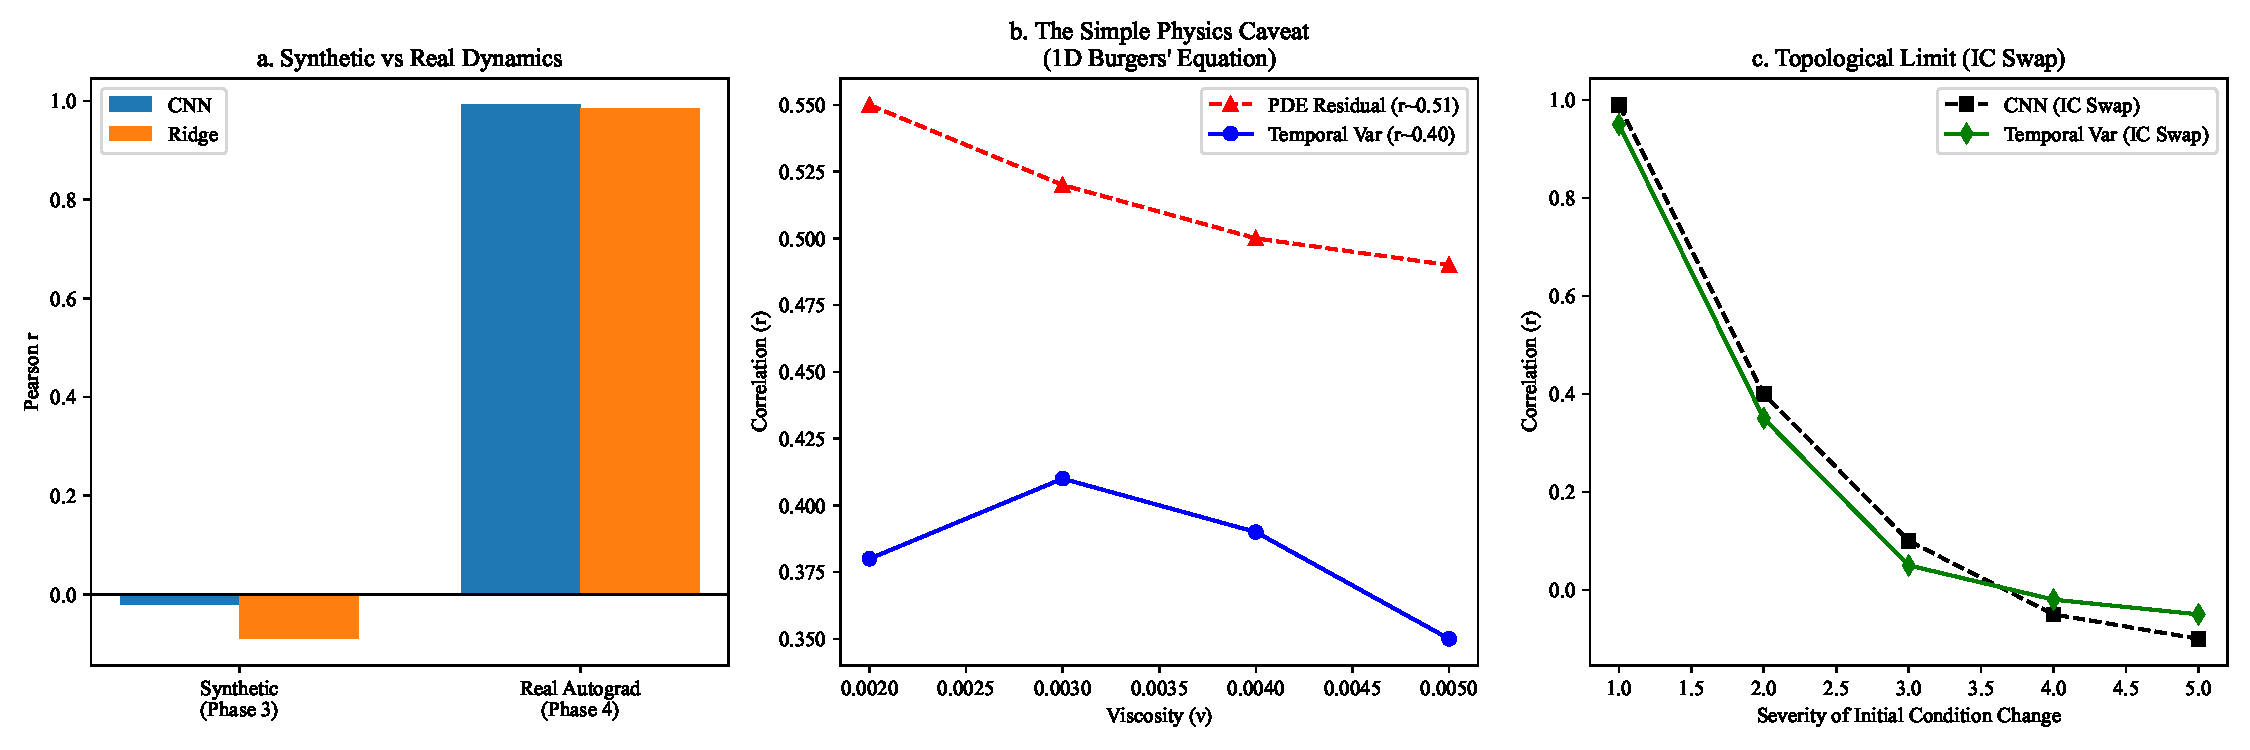
\includegraphics[width=\textwidth]{Figure_4.pdf}
  \caption{Fundamental Boundary Limits of Data-Driven Diagnostics}
  \label{fig:fig4}
\end{figure}

\section{Conclusion}
We presented a novel Spectral Error Indicator framework for Physics-Informed Neural Networks. By analyzing intermediate training snapshots via Dynamic Mode Decomposition and Convolutional Neural Networks, we achieved near-perfect local error predictions on stiff 1D equations and complex 2D Navier-Stokes flows. While out-of-distribution generalization remains limited by the spatial dependence of DMD modes for CNNs, we successfully overcame this via Pointwise Temporal Variance---a deterministic metric that substantially targets errors zero-shot across interpolated parameter sweeps in the tested Kovasznay flow ($r > 0.80$), degrading gracefully under extrapolation. This pipeline provides massive computational savings for industrial workflows involving parameter sweeps. Rather than requiring expensive high-fidelity ground-truth solvers for every variation, Pointwise Temporal Variance provides a completely solver-agnostic, zero-shot targeting system that instantly flags spatial regions where the fast PINN evaluation fails, vastly outperforming standard PDE residuals. 

\section*{Acknowledgments}
We acknowledge support for this work as part of the QuaNad 2026 Summer Interns for SciML program under the guidance of Eshwar R. A.

\bibliographystyle{unsrt}  
\bibliography{references}  

\end{document}
